\documentclass[10pt, a4paper]{article}

\usepackage[a4paper, margin=2cm]{geometry}
\usepackage[english]{babel}
\usepackage{csquotes}
\usepackage{hyperref}
\usepackage[dvipsnames]{xcolor}
\usepackage{ulem}
\usepackage{setspace}
\usepackage{tikz}
\usetikzlibrary{arrows, shapes}
\newlength{\mytw}
\settowidth{\mytw}{A few lines of text in a block}


\usepackage{algorithm} 
\usepackage{algpseudocode}

%\usepackage{hologo}

%\usepackage{float}

%\usepackage{babelbib}

%\usepackage{amsmath}
%\usepackage{amssymb}
%\usepackage{amsthm}

\usepackage{graphicx}
\graphicspath{ {./Pictures/} }

\begin{document}

\pagenumbering{roman} 
\textcolor{white}{ }

\vspace{-1cm}

%\begin{figure}[h]
%	\flushright 
%	\includegraphics[width=5cm]{Bilder/logop}
%\end{figure}

\vspace{1.5cm}
\begin{center}

\sffamily

\fontsize{12pt}{1}{\upshape{}}
	\vspace{2cm}

\fontsize{20pt}{1}{\textbf{PETRINET SIMULATOR}}
	\vspace{0.3cm}

\fontsize{18pt}{1}{\upshape{}}
	\vspace{2.5cm}

\fontsize{14pt}{1}{\upshape{}}
	\vspace{0.2cm}

\fontsize{12pt}{1}{\textbf{Program Documentation}}
	\vspace{0.2cm}

\fontsize{12pt}{1}{\upshape{}}
	\vspace{2.5cm}

\fontsize{18pt}{1}{\upshape{}}
	\vspace{4.5cm}

\fontsize{16pt} {1}{\upshape{}}
	\vspace{1cm}

\fontsize{16pt} {1}{\uline{\textbf{}}}
	\vspace{1cm}

\fontsize{12pt} {1}{\upshape{}}


\end{center}

\thispagestyle{empty}
\newpage
%\afterpage{\blankpage}



 
%\normalem 
% \blankpage

%\textcolor{white}{彩蛋}
\thispagestyle{empty}
\newpage 

\tableofcontents \thispagestyle{plain} \newpage


\pagenumbering{arabic} \rmfamily \onehalfspace 

\section{Manual}
%\label{sec1}
\label{label:introduction}
The Petrinet Simulator is able to display a petrinet and gradually build a reachability graph by firing transitions using the \textit{GraphStream} library\footnote{\url{https://graphstream-project.org/}}. The following picture shows the programs surface:

\begin{center}
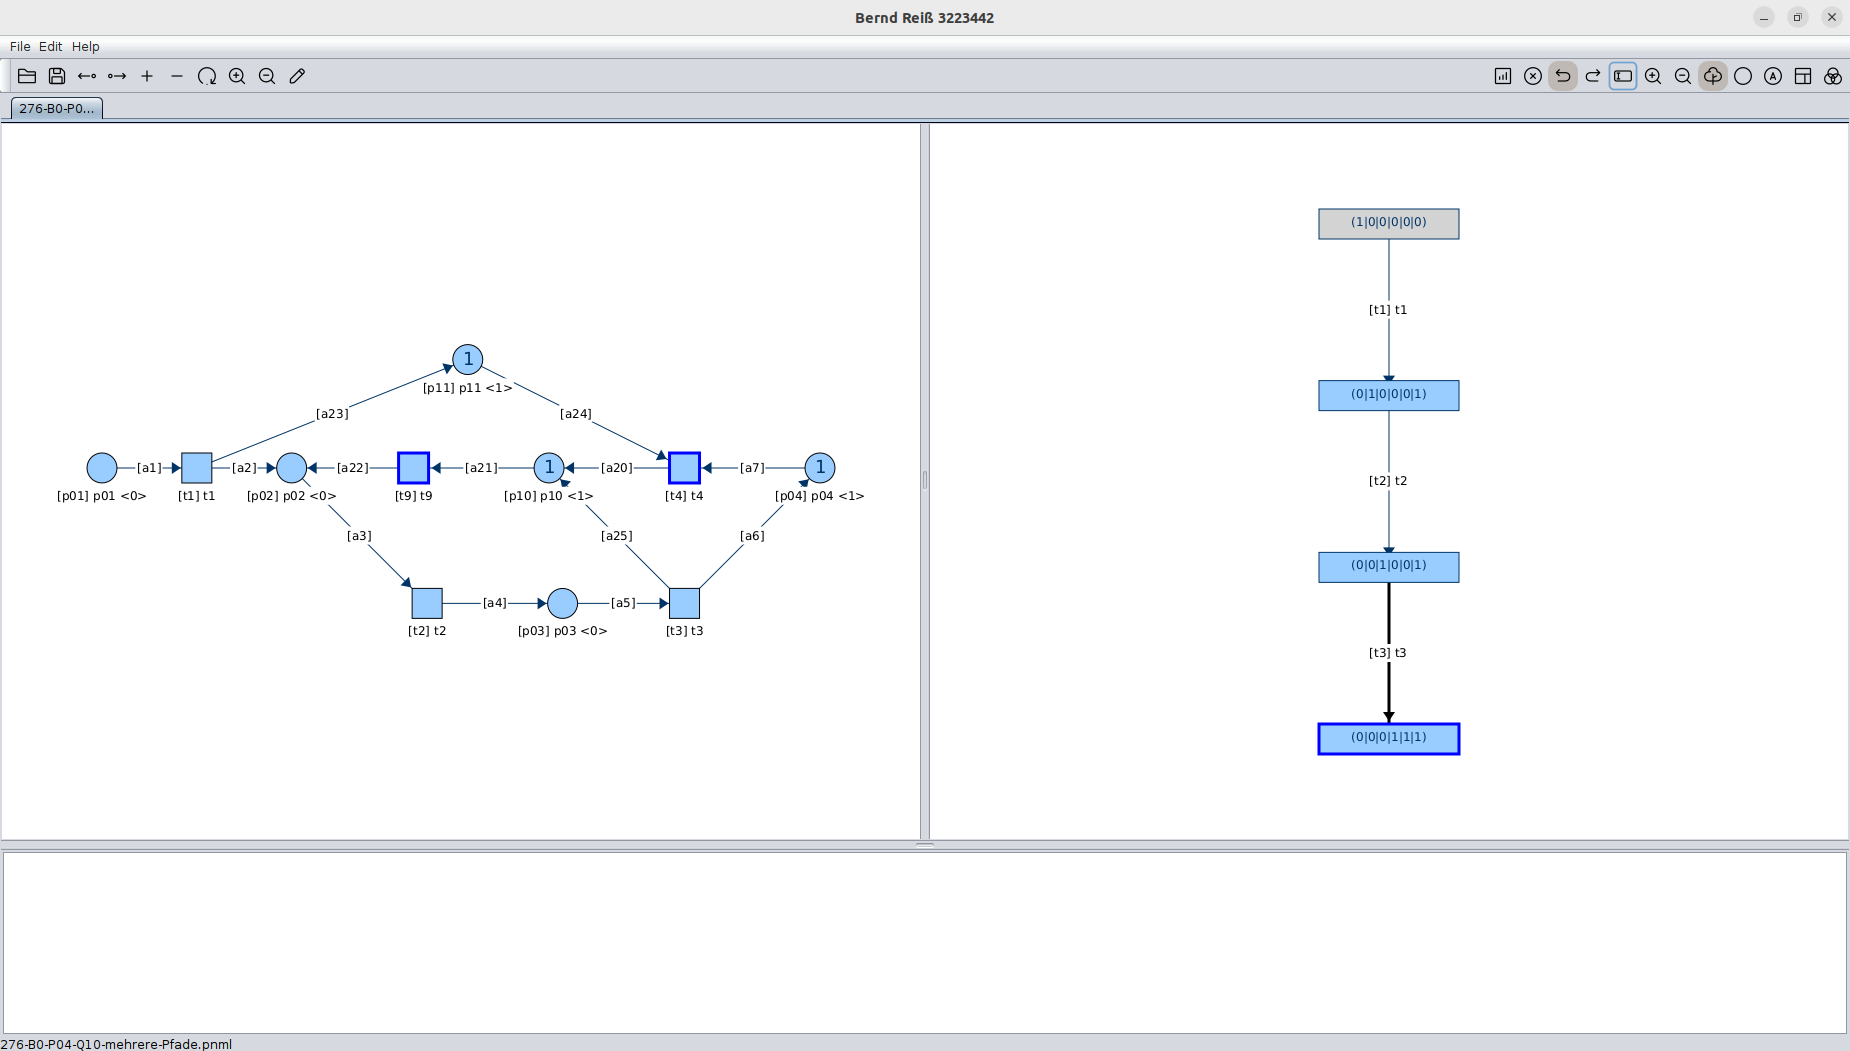
\includegraphics[width=\textwidth]{Pictures/Example_276.png}
\end{center}

In the petrinet on the left activated transitions are marked bold, these transitions can be fired. On the right in the reachability graph the current state is marked bold. Additionally the initial state is marked gray. After performing the boundedness analysis the graphs look like this: 

\begin{center}
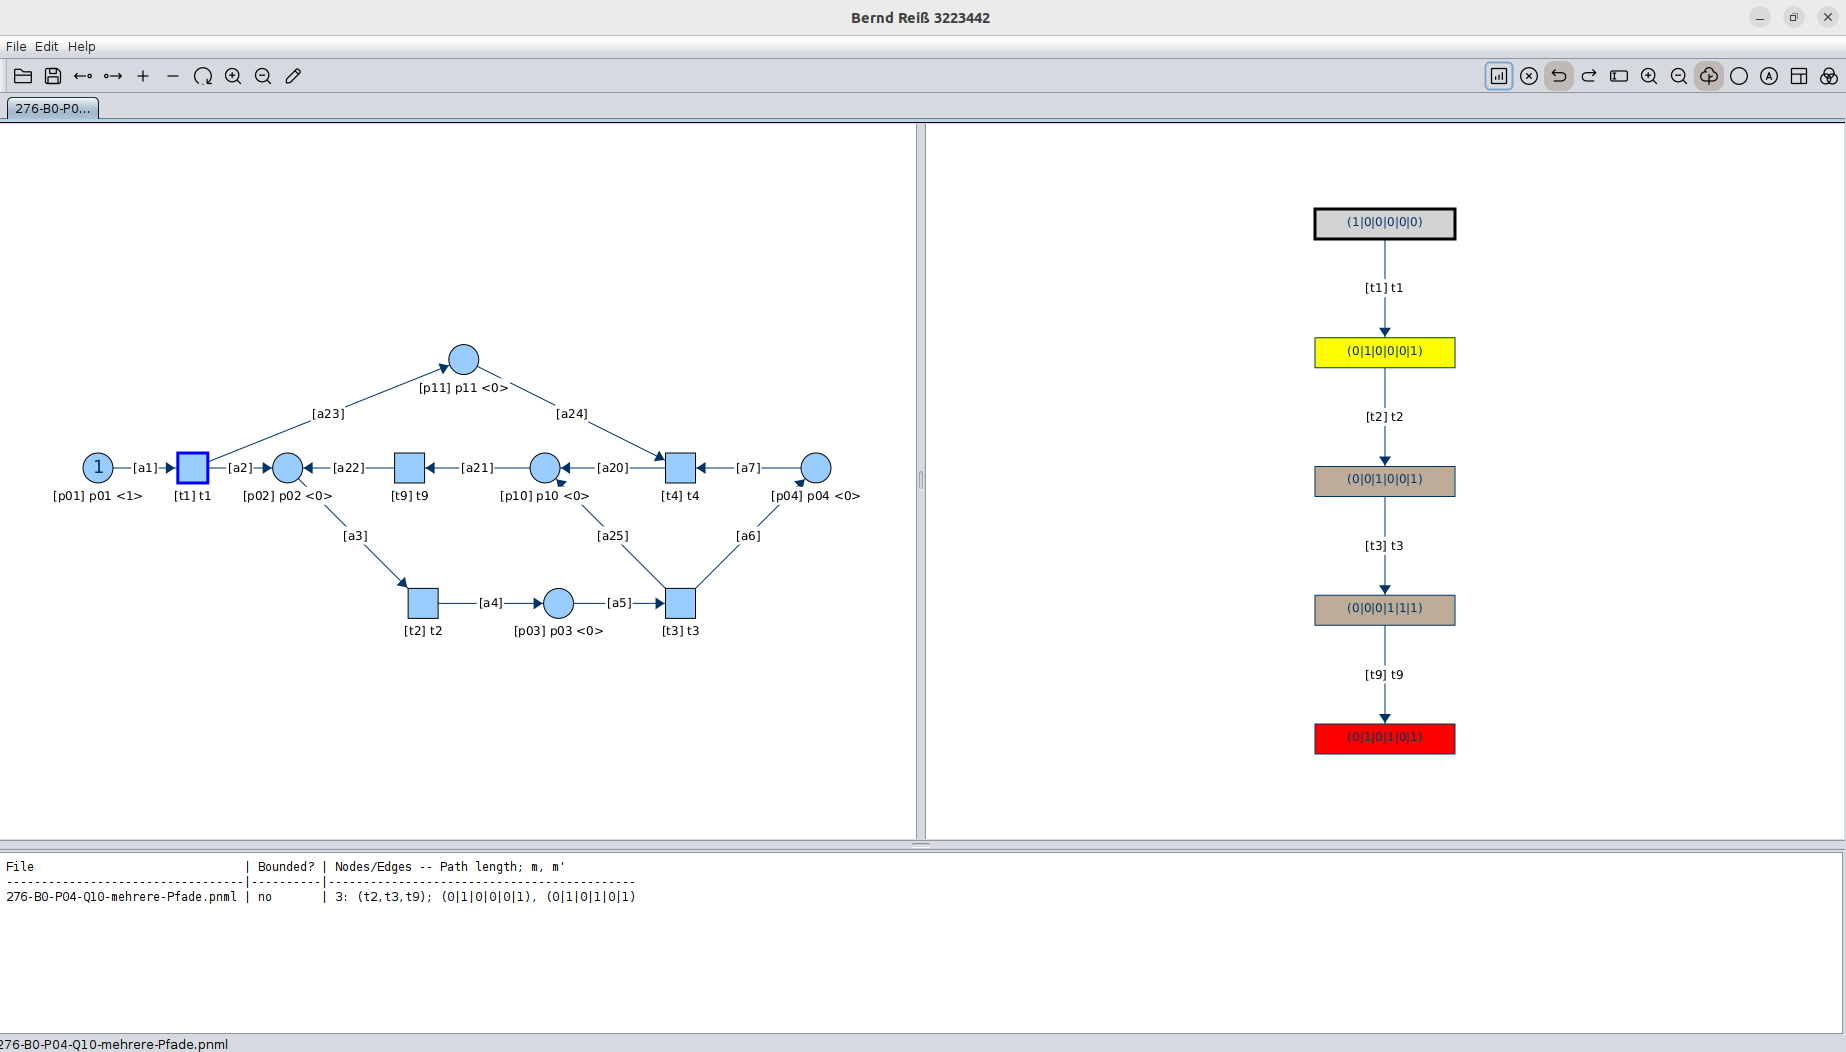
\includegraphics[width=\textwidth]{Pictures/Example_276_analysed.png}
\end{center}

The reachability graph shows whether it encountered a state that signifies that the petrinet is unbounded and marks the beginning (yellow) and ending (red) nodes on the path signifying unboundedness. Any states on the paths between these nodes and between the yellow and intial node are marked also (brown).

The following sections give an overview of additional features implemented in the program and explain the menus and toolbars.

\subsection{Additional features}

\paragraph{Automatic Boundedness Check} By default building the reachability check automatically checks whether the petrinet is bounded or not (see also \ref{label:algorithm}). This can be turned off in the menu \textit{Edit}.

\paragraph{Tabs} A new petrinet can be opened in a new tab. This can be done via the menu \textit{File}.

\paragraph{Undo/Redo} The reachability graph provides undo/redo functionality.

\paragraph{Custom Layouts} The Petrinet Simulator provides two custom layouts: tree layout and circle layout (see \ref{label:layout}). Users can switch between these two and the automatic layout provided by GraphStream.

\paragraph{Editor Mode} Petrinets can be edited in an editor mode (see \ref{label:editor}).


\subsection{Menus}

\subsubsection{File}
\label{label:file}
The \textit{File} menu consists of the following entries:

\begin{itemize}

\item \textbf{New:} opens a new empty file for editing $\rightarrow$ automatically opens the Editor view (see \ref{label:editor}). 
\item \textbf{Open:} opens saved file from directory.
\item \textbf{Open in new Tab:} same as open but in a new tab.
\item \textbf{Reload:} reload the currently opened file.
\item \textbf{Save:} save changes.
\item \textbf{Save as:} save changes and choose directory/name.
\item \textbf{Analyse++:} analyse many petrinets at once. Results are printed in the text area.
\item \textbf{Close:} close currently opened file.
\item \textbf{Exit:} close the program.

\end{itemize}


\subsubsection{Edit}


The \textit{Edit} menu consists of the following entries:


\begin{itemize}
\item \textbf{Open Editor:} opens the Editor.
\item \textbf{Close Editor:} closes the Editor and reverts back to Viewer.
\item \textbf{Change Look and Feel:} change between Nimbus and Metal look and feel.
\item \textbf{Enable Automatic Boundedness Check:} automatically check for boundedness when building the reachabilty graph.
\item \textbf{Disable Automatic Boundedness Check:} do not automatically check for boundedness when building the reachabilty graph.
\end{itemize}

\subsubsection{Help}

The \textit{Help} menu only consists of the element \textit{Info}, which shows information about the Java version used and the user directory.

\subsection{Toolbar Modes}
\label{label:modes}
The program has two distinct toolbar modes: viewer mode and editor mode. This section discusses the two modes and toolbar buttons associated with it. In general the toolbar is fully de- and reattachable (except for the bottom of the program being reserved for the status bar). All icons for the toolbar buttons are taken from \url{https://iconoir.com/}.

\subsubsection{Viewer Mode}

The viewer mode provides functionality for viewing petrinets and building the reachability graph. The toolbar is split into two parts: the petrinet toolbar to the left and the reachability graph toolbar to the right.

\paragraph{Petrinet Toolbar}


\includegraphics[height=0.5cm]{Viewer_Petrinet_Toolbar.png}
\label{label:viewer}

From left to right the buttons provide the following functionality:

\begin{itemize}

\item
\includegraphics[scale=0.4]{../src/resources/images/Toolbar/folder.png}\hspace{0.1cm}\textbf{Load:} see Menu \textit{File} \ref{label:file}.
\item
\includegraphics[scale=0.4]{../src/resources/images/Toolbar/save.png}\hspace{0.1cm}\textbf{Save:} see Menu \textit{File} \ref{label:file}.
\item
\includegraphics[scale=0.4]{../src/resources/images/Toolbar/left.png}\hspace{0.1cm}\textbf{Previous:} open the previous file in the current directory $\rightarrow$ do nothing if current file is the first.
\item
\includegraphics[scale=0.4]{../src/resources/images/Toolbar/right.png}\hspace{0.1cm}\textbf{Next:} open the next file in the current directory $\rightarrow$ do nothing if current file is the last.
\item
\includegraphics[scale=0.4]{../src/resources/images/Toolbar/plus.png}\hspace{0.1cm}\textbf{Increment Place:} increment a marked place by one token.
\item
\includegraphics[scale=0.4]{../src/resources/images/Toolbar/minus.png}\hspace{0.1cm}\textbf{Decrement Place:} decrement a marked place by one token.
\item
\includegraphics[scale=0.4]{../src/resources/images/Toolbar/restart.png}\hspace{0.1cm}\textbf{Reset:} reset the petrinet graph to initial state $\rightarrow$ if place was in-/decremented the initial state is being updated.
\item
\includegraphics[scale=0.4]{../src/resources/images/Toolbar/zoom-in.png}\hspace{0.1cm}\textbf{Zoom in:} zoom into petrinet graph.
\item
\includegraphics[scale=0.4]{../src/resources/images/Toolbar/zoom-out.png}\hspace{0.1cm}\textbf{Zoom out:} zoom out of patrinet graph.
\item
\includegraphics[scale=0.4]{../src/resources/images/Toolbar/edit.png}\hspace{0.1cm}\textbf{Open Editor:} open the Editor (see \ref{label:editor}).
\end{itemize}

\paragraph{Reachbility Graph Toolbar}


\includegraphics[height=0.5cm]{Viewer_Reachability_Toolbar.png}

From left to right the buttons provide the following functionality:
\begin{itemize}
\item
\includegraphics[scale=0.4]{../src/resources/images/Toolbar/stats.png}\hspace{0.1cm}\textbf{Analyse Petrinet:} analyse the petrinet currently opened $\rightarrow$ the reachability graph is built and a pop up window shows whether the petrinet is bounded or unbounded. If the petrinet is unbounded the path signifying unboundedness is marked (see \ref{label:introduction}). 
\item
\includegraphics[scale=0.4]{../src/resources/images/Toolbar/delete.png}\hspace{0.1cm}\textbf{Reset:} delete the reachability graph except for the initial state (marked gray). Also resets the petrinet. 
\item
\includegraphics[scale=0.4]{../src/resources/images/Toolbar/undo.png}\hspace{0.1cm}\textbf{Undo:} undo the last step in the reachability graph. If last step was analysis it is treated as one single step.
\item
\includegraphics[scale=0.4]{../src/resources/images/Toolbar/redo.png}\hspace{0.1cm}\textbf{Redo:} redo the last step in the reachability graph. If last step was analysis it is treated as one single step.
\item
\includegraphics[scale=0.4]{../src/resources/images/Toolbar/input.png}\hspace{0.1cm}\textbf{Clear text area:} clears the text area.
\item
\includegraphics[scale=0.4]{../src/resources/images/Toolbar/zoom-in.png}\hspace{0.1cm}\textbf{Zoom in:} zoom into reachability graph.
\item
\includegraphics[scale=0.4]{../src/resources/images/Toolbar/zoom-out.png}\hspace{0.1cm}\textbf{Zoom out:} zoom out of reachability graph.
\item
\includegraphics[scale=0.4]{../src/resources/images/Toolbar/tree-layout.png}\hspace{0.1cm}\textbf{Tree layout:} organize the reachability graph in a tree layout (see \ref{label:treeLayout}).
\item
\includegraphics[scale=0.4]{../src/resources/images/Toolbar/circle-layout.png}\hspace{0.1cm}\textbf{Circle layout:} organize the reachability graph in a circle layout (see \ref{label:circleLayout}).
\item
\includegraphics[scale=0.4]{../src/resources/images/Toolbar/auto-layout.png}\hspace{0.1cm}\textbf{Automatic Layout:} use the auto layout by GraphStream to organize the reachability graph.
\item
\includegraphics[scale=0.4]{../src/resources/images/Toolbar/layout.png}\hspace{0.1cm}\textbf{Reset Split Panes:} reset the split panes to the default ratio.
\item
\includegraphics[scale=0.4]{../src/resources/images/Toolbar/design.png}\hspace{0.1cm}\textbf{Change Look and Feel:} change between the different look and feels (\textit{Metal} or \textit{Nimbus}).
\end{itemize} 
%\hologo{LaTeX} 
%\ref{sec1}

\subsubsection{Editor Mode}
\label{label:editor}
\paragraph{Petrinet Toolbar}


\includegraphics[height=0.5cm]{Editor_Toolbar.png}

From left to right the buttons provide the following functionality:
\begin{itemize}
\item
\includegraphics[scale=0.4]{../src/resources/images/Toolbar/folder.png}\hspace{0.1cm}\textbf{Load:} see Menu \textit{File} \ref{label:file}.
\item
\includegraphics[scale=0.4]{../src/resources/images/Toolbar/save.png}\hspace{0.1cm}\textbf{Save:} see Menu \textit{File} \ref{label:file}.
\item
\includegraphics[scale=0.4]{../src/resources/images/Toolbar/left.png}\hspace{0.1cm}\textbf{Previous:} see Petrinet Toolbar in Viewer Mode (\ref{label:viewer}).
\item
\includegraphics[scale=0.4]{../src/resources/images/Toolbar/right.png}\hspace{0.1cm}\textbf{Next:} see Petrinet Toolbar in Viewer Mode (\ref{label:viewer}).
\item
\includegraphics[scale=0.4]{../src/resources/images/Toolbar/plus.png}\hspace{0.1cm}\textbf{Increment Place:} see Petrinet Toolbar in Viewer Mode (\ref{label:viewer})..
\item
\includegraphics[scale=0.4]{../src/resources/images/Toolbar/minus.png}\hspace{0.1cm}\textbf{Decrement Place:} see Petrinet Toolbar in Viewer Mode (\ref{label:viewer})..
\item
\includegraphics[scale=0.4]{../src/resources/images/Toolbar/zoom-in.png}\hspace{0.1cm}\textbf{Zoom in:} see Petrinet Toolbar in Viewer Mode (\ref{label:viewer})..
\item
\includegraphics[scale=0.4]{../src/resources/images/Toolbar/zoom-out.png}\hspace{0.1cm}\textbf{Zoom out:} see Petrinet Toolbar in Viewer Mode (\ref{label:viewer})..
\item
\includegraphics[scale=0.4]{../src/resources/images/Toolbar/add-circle.png}\hspace{0.1cm}\textbf{Add Place:} add a place above the left top most element.
\item
\includegraphics[scale=0.4]{../src/resources/images/Toolbar/add-square.png}\hspace{0.1cm}\textbf{Add Transition:} add a transition above the left top most element.
\item
\includegraphics[scale=0.4]{../src/resources/images/Toolbar/erase.png}\hspace{0.1cm}\textbf{Remove Element:} remove the marked element (place or transition).
\item
\includegraphics[scale=0.4]{../src/resources/images/Toolbar/arc.png}\hspace{0.1cm}\textbf{Add Edge:} choose beginning and ending node of an edge to add it $\rightarrow$ beginning and ending nodes have to be of different type (place/transition).
\item
\includegraphics[scale=0.4]{../src/resources/images/Toolbar/remove-edge.png}\hspace{0.1cm}\textbf{Remove Edge:} choose beginning and ending node of an edge to remove it $\rightarrow$ the edge has to exist.
\item
\includegraphics[scale=0.4]{../src/resources/images/Toolbar/label.png}\hspace{0.1cm}\textbf{Add Label:} add label to marked place or transition.
\item
\includegraphics[scale=0.4]{../src/resources/images/Toolbar/eye.png}\hspace{0.1cm}\textbf{Close Editor:} close the Editor and opens the Viewer (see \ref{label:viewer}).
\end{itemize}


\paragraph{Reachability Graph Toolbar}


\includegraphics[height=0.5cm]{Editor_Reachability.png}

From left to right the buttons provide the following functionality:
\begin{itemize}
\item
\includegraphics[scale=0.4]{../src/resources/images/Toolbar/layout.png}\hspace{0.1cm}\textbf{Reset Split Panes:} see Reachability Graph Toolbar in Viewer Mode (\ref{label:viewer}).
\item
\includegraphics[scale=0.4]{../src/resources/images/Toolbar/design.png}\hspace{0.1cm}\textbf{Change Look and Feel:} see Reachability Graph Toolbar in Viewer Mode (\ref{label:viewer}).
\end{itemize}

\section{Design of the Program}


\subsection{General Structure}

The approach of designing this program came from a simplified notion of petrinets. A Petrinet is essentially determined by its places and transitions. The reachability graph in turn represents different petrinets and -- as the name suggests -- the reachability from state to state. The number of tokens on places represent the state of a petrinet and activated transition represent passages between states. These in order are buildings blocks for nodes and edges in the reachability graph. As places and transitions in this implementation of a petrinet simulator know their predecessors and successors they hold all the information needed for a data structure representing a petrinet. Thus the rest of the program essentially revolves around managing places and transitions\footnote{Although in this sense the petrinet model can be seen as a kind of controller, it is still considered to be mainly a data structure, just not as pure as places and transitions might be.}. The job of the reachability graph then is to simply listen to changes in the petrinet. In turn it is also the the job of the graphs to simply listen to changes in the petrinet/reachability graph as they represent their respective data. 

This is where controllers and listeners come in. On a general level it can be noted that controllers control the input provided via the GUI elements and listeners transfer changes in the data model to the GUI components. The program is split into a set of hierarchichally organized controllers. For a general overview of the flow of control please refer to Figure \ref{figure:design}. Double rules signify a GUI component, dashed lines signify interfaces / listeners. The figure demonstrates the basic design of the program and how the essential data models, controllers and GUI components communicate with each other. 

The following sections give a detailed description of how the data models are structured and how controllers and listeners work. Other parts of the program not shown in the figure are discussed in the text also.
\begin{center}
\begin{figure}
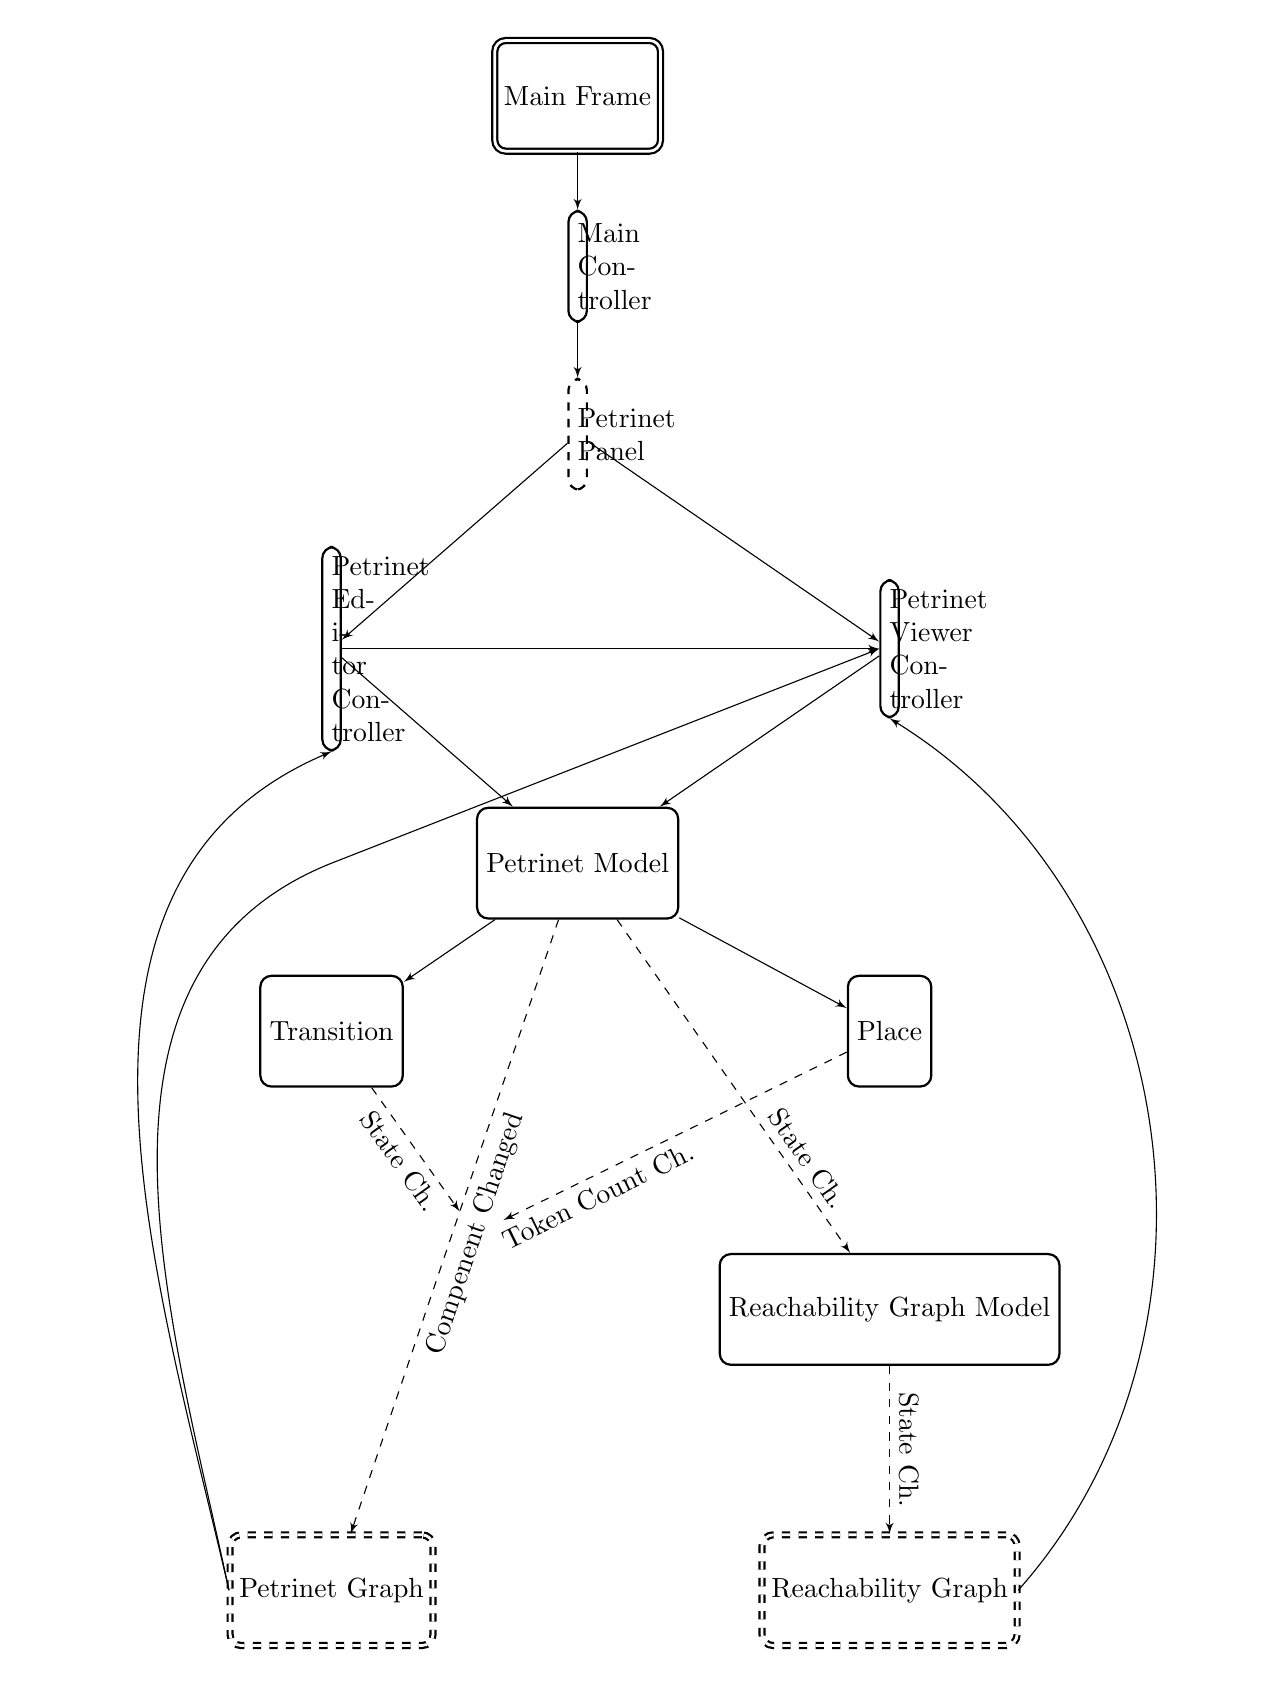
\begin{tikzpicture}
[> = latex', auto,
block/.style ={rectangle,draw=black, thick,
align=flush center, rounded corners,
minimum height=4em},
]
\matrix [column sep=5mm,row sep=7mm]
{
% row 1
&
\node [block, double, double distance=1pt] (mf) {Main Frame}; & \\

% row 2
& 
\node [block, text width=\mytw] (mc) {Main Controller}; & \\

% row 3
& 
 \node[block, dashed, text width=\mytw] (pp) {Petrinet Panel}; & \\

% row 2

\node [block, text width=\mytw] (pec) {Petrinet Editor Controller}; & 
&
\node [block, text width=\mytw] (pvc) {Petrinet Viewer Controller};  \\

% row 1
\node[inner sep = 0pt] (dummy) {};
&
\node [block] (pnm) {Petrinet Model};  \\
% \node[inner sep = 0pt] (dummy) {};
% row 2

\node [block] (tr) {Transition}; &
&
\node [block] (pl) {Place}; & \\

&&\\
&&\\
% row 1
&&
\node [block] (rgm) {Reachability Graph Model}; \\
&&\\
&&\\

%row 4

\node [block, dashed, double, double distance=1pt] (pg) {Petrinet Graph}; &
&\node [block, dashed, double, double distance=1pt] (rg) {Reachability Graph};\\
};

 \draw[->] (mf) -- (mc);
 \draw[->] (mc) -- (pp);
 \draw[->] (pp) -- (pvc); 
 \draw[->] (pp) -- (pec);
 \draw[->] (pvc) -- (pnm); 
 \draw[->] (pec) -- (pnm); 
 \draw[->] (pec) -- (pvc);
 \draw[->] (pnm) -- (pl);
 \draw[->] (pnm) -- (tr);
 \draw[->, dashed] (pnm) -- (pg) node [midway, below, sloped] (cch) {Compenent Changed};
 \draw[->, dashed] (pnm) -- (rgm) node [near end, above, sloped] (sch) {State Ch.};
 \draw[->, dashed] (pl) -- (cch) node [near end, below, sloped] (tcch) {Token Count Ch.};
 \draw[->, dashed] (tr) -- (cch) node [midway, below, sloped] (tsch) {State Ch.};
 \draw[->, dashed] (rgm) -- (rg) node [midway, above, sloped] (rsch) {State Ch.};
 \draw [->, bend right] (pg.west) to[out=20,in=120] (pec.south);
 \draw [->, bend right] (pg.west) to[out=20,in=120] (dummy) -- (pvc.west);
  \draw [->] (rg.east) to[bend right = 50] (pvc.south);
 %\draw [->, bend right] (dummy) -- (pvc.west);
%\draw [->] (pg.west) to[bend right = -90] (pvc.west);
\end{tikzpicture}
\caption{General Design of the Program.}
\label{figure:design}

\end{figure}
\end{center}




\subsubsection{Data Models}

\paragraph{Petrinet Model} It handles everything belonging to the petrinet only. It has functions for modifying the petrinet (such as adding or removing elements) and checks whether an action is valid. If an action is not valid it throws an according \textit{PetrinetException}. The petrinet model holds helper data structures \textit{Place} and \textit{Transition}. There is no data structure for arcs, as they are fully defined via the places and transitions connected to them\footnote{For storing ids belonging to arcs a map is used.}. Rather arcs are defined by elements preceding and succeeding places and transitions. Places contain information about the number of tokens stored in them. Transitions have a status of being activated or not activated.   
\paragraph{Reachability Graph Model} It provides methods for adding/removing states to/from the reachability graph and giving information about the graph. It contains a list of \textit{PetrinetStates}. Such a state contains predecessor and successor states, information about the tokens on the places in the petrinet as well as a state called \textit{m}, being the first state on a path that marks the given state as unbounded. When a new state is added the model checks whether the new state completes a path signifying unboudedness (see \ref{label:algorithm}). If so, the state at the start of the path is remembered by the state and the reachability graph model remembers the last state on the path. The states also store transitions leading up to them and from them. These are stored in lists in a map.
\paragraph{Reachability Graph Undo Queue} This queue records all the steps taken in the reachabilty graph and keeps track of the actions being taken (i.e. whether something has been added). To this end it has its own data structure called \textit{ReachabilityGraphUndoQueueState}. The queue can go back or forward or can be rewinded/reset. If it goes backward, alls steps are undone. Going forward means redoing all steps. The reachability model has methods to stop pushing steps onto the queue. Furthermore steps can be recorded as \enquote{skippable}. A step being skippable means on un-/redo it does not stop but continues going back-/forwards. This enables a multi step process like adding steps when analysing the petrinet to be treated as one big step.  

\subsubsection{Controllers}
There are three controllers in the program: the main controller, the petrinet viewer controller and the petrinet editor controller. Additionally the \textit{PetrinetPanelInterface} serves as an intermediary between the main controller and the other controllers.

\paragraph{Main Controller} On a general level there is a main frame and a number of petrinets in tabs. The task of the main controller is to pass user interactions with elements belonging to the main frame (menus and toolbars) to the petrinet panel that is currently active. If tabs are switched it is also the task of the main controller to restore the state of the toolbar with regards to highlighted buttons for the active petrinet or switching to editor/viewer mode (see \ref{label:modes}). 
\paragraph{Petrinet Panel Interface} This interface forwards messages from the main controller. It also handles clicks and forwards them to either the viewer controller or the editor controller. Additionally it keeps track of the toolbar mode and handles GUI related actions for an instance of a petrinet. 
\paragraph{Petrinet Viewer Controller} This controller manages all clicks on the petrinet when in viewer mode and clicks on the reachability graph. It provides methods for interactions with the petrinet and reachability graph except those pertaining to editing the petrinet.  
\paragraph{Petrinet Editor Controller} This controller manages all clicks on the petrinet when in editor mode. It is tasked with providing functionality when editing the given petrinet. This controller could have been part of the petrinet viewer controller. But because the size of both controllers being combined as one would have been quite big and clicks on transitions are handled differently in viewer and editor mode this solution appeared more manageable.

\subsubsection{Listeners}

\paragraph{Petrinet State Changed Listener} This listener serves as an intermediary between the petrinet model and the reachability graph model. When the petrinet changes states the reachability graph is informed. It distinguishes between states changing because a transition has been fired and changing states because the petrinet has changed $\rightarrow$ in the latter case the reachability graph and its initial state have to be reset.
\paragraph{Petrinet Component Changed Listener} This listener communicates changes in components of the petrinet to the petrinet graph. Whenever elements are added/removed or their attributes are changed it forwards this information.  Because it listens for changes in elements it also listens to the \textit{NumberOfTokensChangedListener} and the \textit{TransitionStateListener} and forwards their events.
\paragraph{Number of Tokens Changed Listener} Part of the data structure \textit{Place} it listens to changes in the number of tokens on the place. If the number changes it informs the petrinet component changed listener. 
\paragraph{Transition State Listener} Part of the data structure \textit{Transition} it listens to changes in the activation state of the transition. If the state changes it informs the petrinet component changed listener.
\paragraph{Reachability State Changed Listener} Listens for changes in the reachability graph model and communicates it to the reachability graph. It contains methods for adding/removing states and also methods for modifying edges.
\paragraph{Toolbar Changed Listener} Listens for events belonging to the un-/redo buttons and the add/remove edge buttons. If events happen the buttons are highlighted accordingly.
\paragraph{Adjust Arrow Heads Listener} This is a special listener for GraphStream. As the arrow heads don't adjust appropriately when adding/removing elements in the graph they need to be adjusted manually. This listener watches for events where arrow heads need to be adjusted.

\subsection{Petrinet Analyser and the Algorithm for Checking Boundedness}
\label{label:algorithm}



The \textit{PetrinetAnalyser} simulates clicking through the transitions of the petrinet and records the results. For this purpose it starts with the initial state and gets all activated transitions. It fires each transition one by one, gets the resulting new state and recursively calls the analyse method. At each firing of a transition the boundedness of the resulting state is checked. If it signifies the petrinet being unbouded the analyser terminates. Otherwise it terminates if it does not encounter new states. It therefore uses a depth first search approach to build the reachability graph step by step.

\begin{algorithm}
\caption{Check if Current State is Bounded in a Petri Net}
\begin{algorithmic}

\Function{CheckIfCurrentStateIsBounded}{}
    \For{each predecessor state $s$ of currentState}
        \State $state \gets$ \Call{CheckIfStateIsBounded}{$s$, new list, currentState}
        \If{$state \neq null$}
            \State $invalidState \gets currentState$
            \State $currentState.setM(state)$
            \State $pathMMarked \gets currentState.getPathFromOtherState(state)$
            \State $pathM \gets state.getPathFromOtherState(initialState)$
            \State \Return $false$
        \EndIf
    \EndFor
    \State \Return $true$
\EndFunction

\Function{CheckIfStateIsBounded}{$state$, $visitedStates$, $originalState$}
    \If{$state$ is in $visitedStates$}
        \State \Return $null$
    \EndIf
    \State Add $state$ to $visitedStates$
    \If{$originalState.isBiggerThan(state)$}
        \State \Return $state$
    \EndIf
    \For{each predecessor state $s$ of $state$}
        \State $newState \gets$ \Call{CheckIfStateIsBounded}{$s$, $visitedStates$, $originalState$}
        \If{$newState \neq null$}
            \State \Return $newState$
        \EndIf
    \EndFor
    \State \Return $null$
\EndFunction

\end{algorithmic}
\end{algorithm}


The actual algorithm for checking the boundedness of a given state is implemented in the reachability graph model itself and is represented by algorithm \ref{algorithm:boundedness}. When a state is added the reachability graph model automatically checks for unboundedness. The state is the \textit{currentState} in the algorithm as any added state becomes the current state in the reachability graph model. As each instance of the petrinet state model knows its predecessors it can search for states that mark the current state as unbounded $\rightarrow$ the algorithm loops through them for the current state and calls the \textit{CHECKIFSTATEISBOUNDED} method for every one of them. This medhod in turn loops through every predecessor of the state passed to it and calls itself recursively. The base case terminating the recursive loop is if the state has already been visitied or if it signifies that the given petrinet is unbounded. To this end the petrinet state model implements a method called \textit{isBiggerThan} that takes a state as a parameter and returns whether the number of tokens on any place is bigger while the tokens on all the other places are the same or bigger also. The algorithm checks the original state (the current in the reachability graph model) and checks it against the state currently passed to the method. This means by performing a depth first search all states in the reachability graph model are checked iteratively until an \textit{m} is found or all states have been checked.


\begin{algorithm}
\caption{Analyse State in a Petrinet}
\label{algorithm:analyser}
\begin{algorithmic}

\Function{AnalyseState}{$state$, $visited$}

    \If{not $bounded$}
    	\State \Return
    \EndIf
    \If{$state$ is in $visited$}
        \State \Return
    \EndIf
    \State $numberOfNodes \gets numberOfNodes + 1$
    \State Add $state$ to $visited$
    \State $petrinet.setState(state)$

    \For{each activated transition $t$ in $petrinet$}
        \State $petrinet.fireTransition(t)$
        \State $stateBounded \gets reachabilityGraphModel.checkIfCurrentStateIsBounded()$
        \If{not $stateBounded$}
            \State $bounded \gets false$
            \State \Return
        \EndIf
        \State $numberOfEdges \gets numberOfEdges + 1$
        \State \Call{AnalyseState}{$reachabilityGraphModel.getCurrentPetrinetState()$, $visited$}
        \State $reachabilityGraphModel.setCurrentState(state)$
        \State $petrinet.setState(state)$
    \EndFor
\EndFunction

\end{algorithmic}
\end{algorithm}



Algorithm \ref{algorithm:analyser} shows how the \textit{PetrinetAnalyser} works. All the analyser has to do is start from the initial state and simulate all possible configurations of the petrinet at hand. It iteratively performs a depth first approach of firing all transitions $\rightarrow$ for each state it loops over all activated transitions, fires them and calls the analyse function for the resulting new state in turn firing all activated transitions in this new state. It does so until all configurations have been exhausted, the reachability model informs the analyser that the petrinet is unbounded or the petrinet has been found unbounded in another configuration (this what the variable \textit{bounded} keeps track of). If the petrinet is unbounded the analyser updates the reachability graph by resetting it to the initial state and only firing the transitions leading up to and including the path marking the petrinet unbouded. This way only the relevant information is shown in the reachability graph.


\subsection{Layout}
\label{label:layout}

The program supports three layouts: two custom layouts and the automatic layout\footnote{see Automatic layout at \url{https://graphstream-project.org/doc/Tutorials/Graph-Visualisation/1.0/}} provided by GraphStream. Only the two custom layouts are discussed in this section.

\subsubsection{Tree Layout}
\label{label:treeLayout}

The tree layout organizes nodes in the reachability graph as a tree. The level in which a node goes into is defined by the length of the path from the initial node and is defined for each state in the class \textit{PetrinetState} and therefore provided to the graph whenever a state is added. On each level the nodes are ordered by their proximity to the parent in the level above $\rightarrow$ nodes should be near below the parent node so edges don't intersect too much with other nodes. Unfortunately this does not prevent intersecting edges altogether. For example if a node has a child directly below and the child has another child directly below and the child of the child has an edge to the grandparent the edge between the grandchild and the grandparent will intersect the child. For this reason adding a new node to the tree performs two additional checks: \textit{checkEdgeIntersection} and \textit{spreadSprites}. The former checks whether any edges intersect with any nodes. If so the nodes are pushed to the left or right according to their position on the level. This is repeated until no edges intersect nodes anymore or until the function has looped 20 times. The latter checks three cases: parallel edges and crossing edges. On parallel edges the sprites need to be moved because they are almost guaranteed to cross each other. This is easy since the default position of sprites is in the middle and can be shifted accordingly. Crossing edges are more tricky. An additional check has to be performed to check whether the sprites actually intersect. To this end the \textit{reachabilityGraphLayout} package provides data structures and functions to work with rectangles. The layout may not solve all issues but in most cases it provides a pleasant experience.

\subsubsection{Circle Layout}
\label{label:circleLayout}

This layout organizes nodes around a circle -- or to be more precise an ellipse. Initially the nodes are ordered by level. Just putting them around a circle would lead to level clusters and most importantly edges clustering at the circles scope. To avoid clusters the initial ordering of nodes is spread evenly around the circle by a certain ratio\footnote{For a more in depth explanation of how the algorithm works please refer to the comments in the source code.}. The ratio to which nodes are spread around the circle can be modified by clicking the circle layout button repeatedly.

%\subsection{Packages}

%\subsubsection{control}

%\subsubsection{core}
%\subsubsection{exceptions}
%\subsubsection{gui}
%\subsubsection{listeners}
%\subsubsection{reachabilityGraphLayout}
%\label{label:package:layout}
%\subsubsection{util}


\newpage
%\begin{table}[t]

%\centering


%\begin{tabular}{| c | c | c | c |}
%\hline
%		& Hobbit		& Ringträger		& Gemeinschaft des Ringes	\\ \hline\hline

%\end{tabular}

%\caption{Verschiedene Charaktere und Gruppierungen in \textit{Der Herr der Ringe}.}
%\label{tab:LOTR}

%\end{table}


%\cite{jamesetal13}

 
%\bibliographystyle{babplain-fl}

%\bibliography{Literatur}

\end{document}
